\documentclass[border=4pt]{standalone}
\usepackage{tikz}
\usetikzlibrary{arrows.meta,shapes.geometric}

\begin{document}
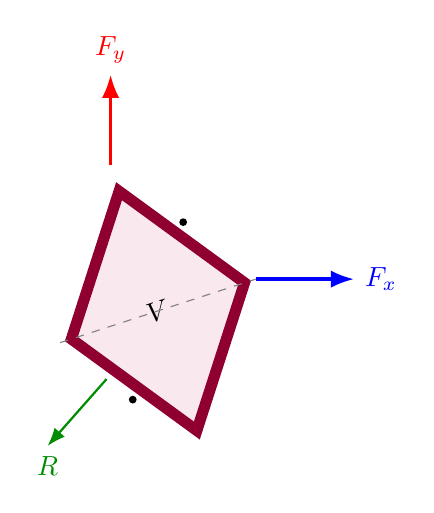
\begin{tikzpicture}[>=Latex]
  \node[diamond,aspect=.72,draw=purple!75!black,line width=4pt,fill=purple!9,
    minimum width=24mm,minimum height=34mm,inner sep=2pt,
    outer xsep=3pt,outer ysep=7pt,rotate=18] (cell) at (0,0) {$V$};

  \draw[dashed,gray] (cell.west) -- (cell.east);
  \fill[black] (cell.north east) circle (1.4pt);
  \fill[black] (cell.south west) circle (1.4pt);
  \draw[->,very thick,red] (cell.north) -- ++(0,1.15) node[above] {$F_y$};
  \draw[->,very thick,blue] (cell.east) -- ++(1.25,0) node[right] {$F_x$};
  \draw[->,thick,green!55!black] (cell.215) -- ++(-.75,-.85) node[below] {$R$};
\end{tikzpicture}
\end{document}
